% asset_id: AS1BinomialExpansionTIKZ-001
% source: CCEA AS1 Sequences and series specification boundary;
%         Dr Frost Maths P1 Chapter 8 Binomial Expansion evidence
% related_lesson_section: Core Theory 8.8; Exam Technique 13.1; Worked Examples 6-9
% purpose: Create a clean coefficient table for the general term
%          \binom{n}{r}a^{n-r}b^r in the finite binomial expansion.
% linked_LOs: AS1-SS-LO001, AS1-SS-LO002

\documentclass[tikz,border=8pt]{standalone}

\usepackage{amsmath}
\usepackage{tikz}
\usetikzlibrary{positioning, arrows.meta, calc}

\begin{document}

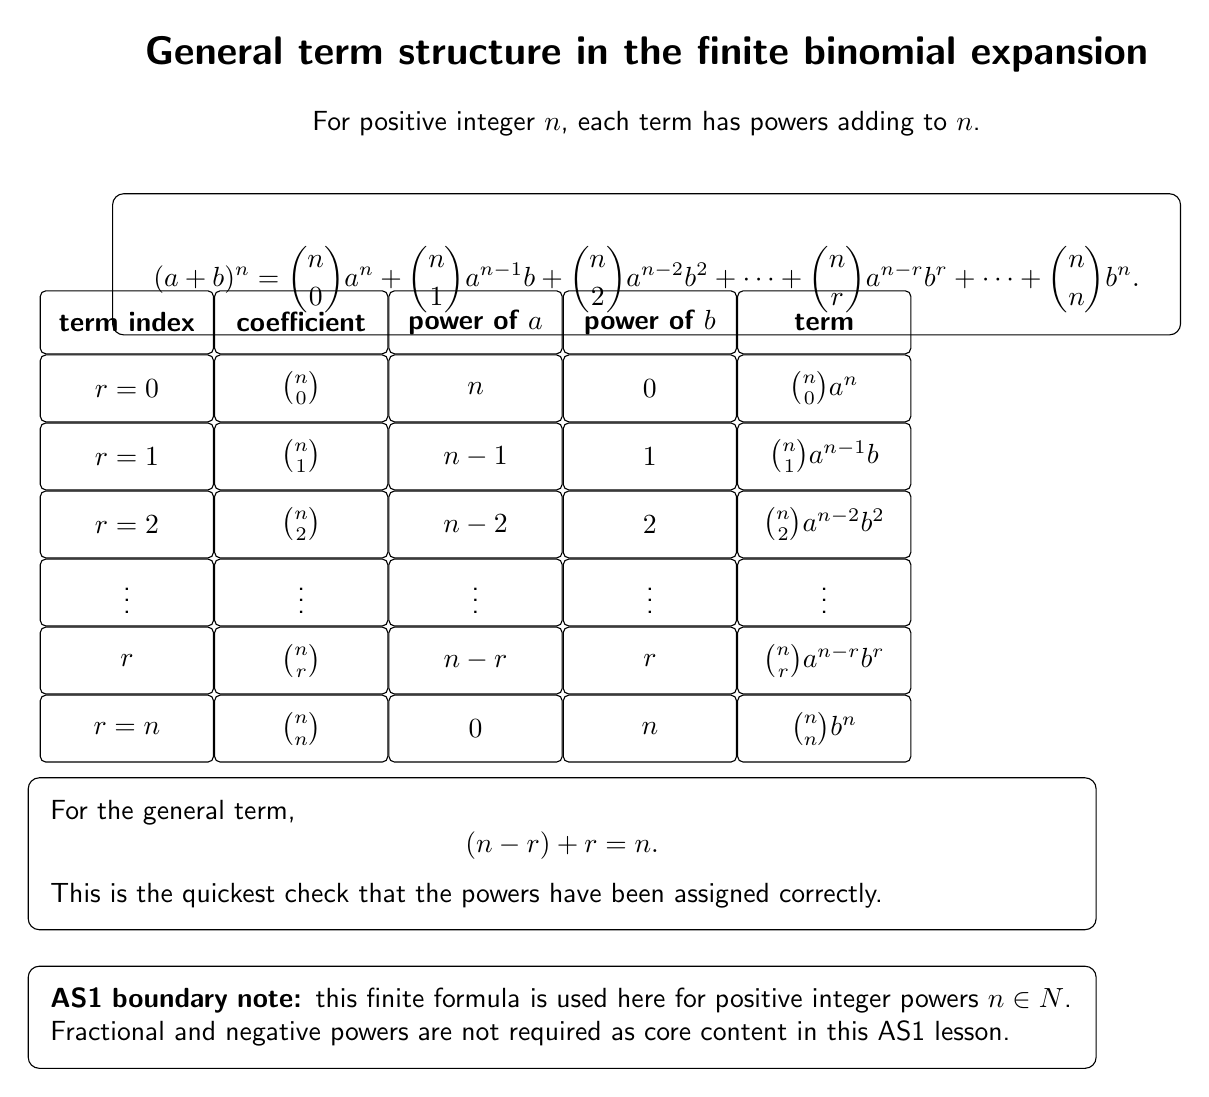
\begin{tikzpicture}[
    font=\sffamily,
    header/.style={draw, rounded corners=2pt, minimum height=0.8cm, align=center, font=\sffamily\bfseries},
    cell/.style={draw, rounded corners=2pt, minimum height=0.85cm, align=center},
    note/.style={draw, rounded corners=4pt, align=left, inner sep=8pt, text width=13cm},
    arrow/.style={-{Latex[length=3mm]}, thick}
]

\node[font=\sffamily\bfseries\Large, align=center] (title) at (0,0)
{General term structure in the finite binomial expansion};

\node[font=\sffamily\normalsize, align=center, below=0.25cm of title] (subtitle)
{For positive integer \(n\), each term has powers adding to \(n\).};

\node[note, below=0.6cm of subtitle] (formula) {
\[
(a+b)^n
=
\binom{n}{0}a^n
+
\binom{n}{1}a^{n-1}b
+
\binom{n}{2}a^{n-2}b^2
+
\cdots
+
\binom{n}{r}a^{n-r}b^r
+
\cdots
+
\binom{n}{n}b^n .
\]
};

\coordinate (start) at (-6.6,-3.4);
\def\wA{2.2}\def\wB{2.2}\def\wC{2.2}\def\wD{2.2}\def\wE{2.2}

\node[header, minimum width=\wA cm] (h1) at ($(start)+(0,0)$) {term index};
\node[header, minimum width=\wB cm, right=0cm of h1] (h2) {coefficient};
\node[header, minimum width=\wC cm, right=0cm of h2] (h3) {power of \(a\)};
\node[header, minimum width=\wD cm, right=0cm of h3] (h4) {power of \(b\)};
\node[header, minimum width=\wE cm, right=0cm of h4] (h5) {term};

\node[cell, minimum width=\wA cm, below=0cm of h1] (r0a) {\(r=0\)};
\node[cell, minimum width=\wB cm, right=0cm of r0a] (r0b) {\(\binom{n}{0}\)};
\node[cell, minimum width=\wC cm, right=0cm of r0b] (r0c) {\(n\)};
\node[cell, minimum width=\wD cm, right=0cm of r0c] (r0d) {\(0\)};
\node[cell, minimum width=\wE cm, right=0cm of r0d] (r0e) {\(\binom{n}{0}a^n\)};

\node[cell, minimum width=\wA cm, below=0cm of r0a] (r1a) {\(r=1\)};
\node[cell, minimum width=\wB cm, right=0cm of r1a] (r1b) {\(\binom{n}{1}\)};
\node[cell, minimum width=\wC cm, right=0cm of r1b] (r1c) {\(n-1\)};
\node[cell, minimum width=\wD cm, right=0cm of r1c] (r1d) {\(1\)};
\node[cell, minimum width=\wE cm, right=0cm of r1d] (r1e) {\(\binom{n}{1}a^{n-1}b\)};

\node[cell, minimum width=\wA cm, below=0cm of r1a] (r2a) {\(r=2\)};
\node[cell, minimum width=\wB cm, right=0cm of r2a] (r2b) {\(\binom{n}{2}\)};
\node[cell, minimum width=\wC cm, right=0cm of r2b] (r2c) {\(n-2\)};
\node[cell, minimum width=\wD cm, right=0cm of r2c] (r2d) {\(2\)};
\node[cell, minimum width=\wE cm, right=0cm of r2d] (r2e) {\(\binom{n}{2}a^{n-2}b^2\)};

\node[cell, minimum width=\wA cm, below=0cm of r2a] (ella) {\(\vdots\)};
\node[cell, minimum width=\wB cm, right=0cm of ella] (ellb) {\(\vdots\)};
\node[cell, minimum width=\wC cm, right=0cm of ellb] (ellc) {\(\vdots\)};
\node[cell, minimum width=\wD cm, right=0cm of ellc] (elld) {\(\vdots\)};
\node[cell, minimum width=\wE cm, right=0cm of elld] (elle) {\(\vdots\)};

\node[cell, minimum width=\wA cm, below=0cm of ella] (rra) {\(r\)};
\node[cell, minimum width=\wB cm, right=0cm of rra] (rrb) {\(\binom{n}{r}\)};
\node[cell, minimum width=\wC cm, right=0cm of rrb] (rrc) {\(n-r\)};
\node[cell, minimum width=\wD cm, right=0cm of rrc] (rrd) {\(r\)};
\node[cell, minimum width=\wE cm, right=0cm of rrd] (rre) {\(\binom{n}{r}a^{n-r}b^r\)};

\node[cell, minimum width=\wA cm, below=0cm of rra] (rna) {\(r=n\)};
\node[cell, minimum width=\wB cm, right=0cm of rna] (rnb) {\(\binom{n}{n}\)};
\node[cell, minimum width=\wC cm, right=0cm of rnb] (rnc) {\(0\)};
\node[cell, minimum width=\wD cm, right=0cm of rnc] (rnd) {\(n\)};
\node[cell, minimum width=\wE cm, right=0cm of rnd] (rne) {\(\binom{n}{n}b^n\)};

\node[note, below=1.05cm of rrc, xshift=1.1cm] (powersum) {
For the general term,
\[
(n-r)+r=n.
\]
This is the quickest check that the powers have been assigned correctly.
};

\node[note, below=0.45cm of powersum] (boundary) {
\textbf{AS1 boundary note:}
this finite formula is used here for positive integer powers \(n\in\mathbb{N}\).
Fractional and negative powers are not required as core content in this AS1 lesson.
};

\end{tikzpicture}

\end{document}
